\documentclass[a4paper,11pt]{article}

% Pacotes Principais -----------------------------------------------------------
\usepackage[portuges,brazil]{babel}
\usepackage[utf8]{inputenc}

% Formatação de capítulos ------------------------------------------------------
%\usepackage[Sonny]{fncychap}
%\usepackage{fncychap}
\usepackage{capitulos}

% Figuras e Imagens ------------------------------------------------------------
\usepackage{graphicx}
% Figuras lado a lado
\usepackage{epsfig}
\usepackage{subfigure}

% Utilizar H para inserir as imagens REALMENTE onde eu desejo
\usepackage{float}

% Fontes -----------------------------------------------------------------------
\usepackage[T1]{fontenc}
\usepackage{pslatex}

% Simbolos ---------------------------------------------------------------------
\usepackage{textcomp}
\usepackage{bbding}

% Tabelas ----------------------------------------------------------------------
%\usepackage{multicol}
\usepackage{multirow}
% Colorir a tabela
\usepackage{colortbl}
% Pacote hhline corrige os bugs das linhas que não aparecem com o colortbm
\usepackage{hhline}
% Tabelas com colunas de largura auto ajustável
\usepackage{tabularx}
% Notas de rodapé em tabelas (Pode-se usar o ambiente longtable também -
% Pesquisar exemplo com longtable)
\usepackage{threeparttable}
% Tabelas grandes
\usepackage{supertabular}

% Glossário --------------------------------------------------------------------
\usepackage[portuguese,noprefix]{nomencl}
\usepackage{makeglo}

% Outros pacotes ---------------------------------------------------------------
\usepackage{noitemsep}

% Comentários em bloco
\usepackage{verbatim}

% Hiperlinks
\usepackage{hyperref}

% Orientação de página
\usepackage{lscape}

% utilitários matemáticos
\usepackage{amsmath}
\usepackage{icomma}

% Evita o problema "too many unprocessed floats", colocando os campos
% 'flutuantes' em suas respectivas seções
\usepackage[section]{placeins}

% Referências ------------------------------------------------------------------
\usepackage[abbr]{harvard}	% As chamadas são sempre abreviadas
\harvardparenthesis{square}	% Colchetes nas chamadas
\harvardyearparenthesis{round}	% Parêntesis nos anos das referências
\renewcommand{\harvardand}{e}	% Substituir "&" por "e" nas referências

% Comandos gerais --------------------------------------------------------------
\newcommand{\titulo}{Sistemas de Tempo Real}
\newcommand{\autor}{Diogo Leite Rebouças}

% Configuração da fonte
%\renewcommand{\familydefault}{\sfdefault}

% Margens ----------------------------------------------------------------------
\setlength{\oddsidemargin}{3.5cm}
\setlength{\evensidemargin}{2.5cm}
\setlength{\textwidth}{15cm}
\addtolength{\oddsidemargin}{-1in}
\addtolength{\evensidemargin}{-1in}

\setlength{\topmargin}{2.0cm}
\setlength{\headheight}{1.0cm}
\setlength{\headsep}{1.0cm}
\setlength{\textheight}{22.7cm}
\setlength{\footskip}{1.0cm}
\addtolength{\topmargin}{-1in}

% Glossário --------------------------------------------------------------------
\makeglossary

% Capítulos --------------------------------------------------------------------
% Não aparecer o número na primeira página dos capítulos
\newcommand{\mychapter}[1]{\chapter{#1}\thispagestyle{empty}}
\newcommand{\mychapterstar}[1]{\chapter*{#1}\thispagestyle{empty}}

% Comandos matemáticos ---------------------------------------------------------
% Implicação em fórmulas
\newcommand{\implica}{\quad\Rightarrow\quad} %Meio de linha
\newcommand{\implicafim}{\quad\Rightarrow}   %Fim de linha
\newcommand{\tende}{\rightarrow}

% Fração com parenteses
\newcommand{\pfrac}[2]{\parent{\frac{#1}{#2}}}

% Transformada de Laplace e transformada Z
\newcommand{\lapl}{\pounds}
\newcommand{\transfz}{\mathcal{Z}}

% Sequências
\newcommand{\sequencia}[4]{$#1_{#2}$, $#1_{#3}$, \ldots, $#1_{#4}$}

% Outros ----------------------------------------------------------------------
\newcommand{\chave}[1]{\left\{#1\right\}}
\newcommand{\colchete}[1]{\left[#1\right]}
\newcommand{\parent}[1]{\left(#1\right)}

\newcommand{\rhoagua}{\rho_{\tiny \text{\tiny H}_2\text{\tiny O}}}

\let\D\displaystyle
\newcommand{\reg}{\textsuperscript{\textregistered}}
\newcommand{\soft}{\textit{software}}
\newcommand{\Soft}{\textit{Software}}

% Imagens exportadas pelo gnuplot ----------------------------------------------
\graphicspath{{imgs/eps/}}


\begin{document}

\begin{table}[H]
\centering
\begin{tabular}{cl}
% Primeira Linha
\multirow{7}{*}
{

\includegraphics[width=1.65cm]{imgs/uern}
} & \\
& Governo do Estado do Rio Grande do Norte\\
% Segunda Linha
& Secretaria de Estado da Educação, da Cultural e dos Desportos -- SECD\\
% Terceira Linha
& {\sc Universidade do Estado do Rio Grande do Norte -- UERN}\\
% Quarta Linha
& Pró-Reitoria de Ensino e Graduação -- PROEG\\
% Quinta Linha
& Ciências da Computação -- Reposição da 1\textordfeminine\ Avaliação (10
  pontos)\\
& 
\end{tabular}
\end{table}

\begin{center}
\large
\uline{Expectativa de Respostas}
\end{center}

\section*{Questão 1 (2 pontos)}
Quando falamos sobre a representação da informação, mostramos que existem dois
tipos de representação de imagens. Cite quais são esses dois tipos de
representação e determine suas características e aplicações.

\vspace{0.25cm}

Os dois tipos de representação são: a representação no formato vetorial e a
representação no formato matricial. 

No formato vetorial, as imagens são constituídas por segmentos de retas e curvas
que possuem características bem definidas de cor, tamanho e espessura, por
exemplo. Este tipo de representação faz uso de planos de coordenadas e é muito
utilizada para modelagem geométrica.

Já na representação matricial as imagens são subdivididas em pequenas regiões,
denominadas de elementos de imagem (ou {\it pixels}) e cada uma dessas pequenas
regiões é codificada através de um modelo cores, como RGB ou RGBA. Quanto maior
for o número de bits utilizado no modelo de cores, maior será a quantidade de
informação de cor armazenada pela imagem e, consequentemente, maior será o
arquivo final.

\pagebreak

\section*{Questão 2 (1 ponto)}
Durante o processo de conversão A/D, devemos determinar o tipo de quantização a
ser utilizada e o número de bits para se representar cada amostra do sinal.
Baseado nessas informações, responda as alternativas abaixo:

\begin{itemize}
    \item [a)] Cite e determine as características dos tipos de quantização
explicados em sala de aula.
\end{itemize}

Existem basicamente dois tipos de quantização: a quantização linear e a
quantização logarítmica.

Na quantização linear, o quantum $\Delta Q$ possui tamanho fixo e os níveis
de quantização são igualmente espaçados. Além disso, o erro de quantização é de
aproximadamente $e = \Delta Q/2$ e as amostras com menor amplitude são mais
penalizadas por esse erro. 

Na quantização logarítmica, o sinal deve ser transformado para a escala
logarítmica de modo que os níveis de quantização não fiquem mais igualmente
espaçados. Essa característica faz com que o erro de quantização diminua
consideravelmente e se torne aproximadamente constante.

\begin{itemize}
    \item [b)] Determine qual será a velocidade mínima ({\bf em Kbit/s}) que um
canal deve assegurar para que haja uma transmissão sem perda de um sinal
digital, obtido a partir de um processo de digitalização (conversão A/D) de um
sinal de voz de 4,5 KHz. Cada amostra deve ser representada por 16 bits.
\end{itemize}

Obedecendo o critério de Nyquist, tem-se:

\[
\omega = 4,5\ \text{KHz}\qquad \Longrightarrow \qquad 2\omega = 9\ \text{KHz}
\]

Arredondando para um valor superior, tem-se a taxa de amostragem ($T_{\tiny
X}$):

\[
T_{\tiny X} = 10\ \text{KHz}
\]

Como cada amostra deve ser representada por 16 bits, então a largura de banda do
canal ($B$) deverá ser de, no mínimo:

\[
B = 160\ \text{Kbps}
\]

\pagebreak

\section*{Questão 3 (1 ponto)}
Sabemos que a criação de imagens, sons e vídeos no formato digital traz
benefícios até mesmo quando o produto final for distribuído em mídia analógica e
que esses recursos estão intimamente relacionados com o conceito de {\bf
multimídia}. Assim sendo, responda:

\begin{itemize}
    \item[a)] O que é multimídia?
\end{itemize}

Multimídia são todos os programas e sistemas em que a comunicação entre o homem
e o computador se dá através de múltiplos meios de representação da informação
(som, imagem, animações \ldots)

\begin{itemize}
    \item[b)] Quais são as principais características dos arquivos multimídia?
\end{itemize}

Os arquivos multimídia possuem características de acesso não linear, em que a
informação é rapidamente acessível e não há uma sequência de tempo como a
leitura de um livro; de interatividade, em que o usuário atua como participante
da atividade computacional; e de integração inter-aplicativos, como por exemplo
na integração de um sistema de gestão de estoque com um banco de dados.

\pagebreak

\section*{Questão 4 (2 pontos)}
Mostramos em sala de aula que existem três tipos de produtos multimídia:
títulos, aplicativos e sítios. Baseado nessas informações, responda:

\begin{itemize}
    \item[a)] Quais são as principais diferenças entre os {\bf aplicativos com
interface multimídia} e os {\bf aplicativos multimídia}?
\end{itemize}

De maneira resumida pode-se dizer que os aplicativos com interface multimídia
são aqueles desenvolvidos em ambientes de programação e que fazem uso de
recursos gráficos e sonoros para interagir com o usuário. Já os aplicativos
multimídia são aqueles que processam a informação multimídia, geralmente em
tempo real. Neste caso, a multimídia deixa de ser um recurso de interface e
passa a ser objeto de processamento do aplicativo.

\begin{itemize}
    \item[b)] O que são sítios? Quais são os possíveis materiais que constituem
um sítio?
\end{itemize}

Sítios são hipermídias armazenadas em servidores Web que podem ser visualizadas
remotamente (máquinas clientes) através de programas navegadores ({\it
browsers}). Normalmente os sítios são escritos em HTML e a navegação se dá
através de hiperligações, podendo conter material multimídia, principalmente ao
se utilizar {\it plugins}.

Os possíveis materiais que constituem os sítios são: páginas hipertexto,
material gráfico e de multimídia, outros tipos de documentos a serem
distribuídos, arquivos de trabalho utilizados pelo servidor e {\it softwares}
ativos, tais como ActiveX, JavaScript e Ajax.

\pagebreak

\section*{Questão 5 (2 pontos)}
Falamos em sala de aula que, para criar qualquer tipo de produto multimídia,
devemos considerar os aspectos relacionados aos {\bf direitos autorais} do
material que utilizamos. Sabendo disso, cite quais são os principais tipos de
restrições (limitações) a serem consideradas.

\vspace{0.25cm}

As principais restrições relacionadas aos direitos autorais são: limitações na
forma de distribuição, em que pode-se permitir a reprodução do vídeo mas não do
áudio; limitações de prazos de utilização; limitações quanto à transferência do
material à terceiros; limitações quanto às regiões de comercialização e
limitações quanto à edição e processamento do material.

\pagebreak

\section*{Questão 6 (2 pontos)}
Uma imagem, representada no {\bf formato matricial}, semelhante à Fig.
\ref{fig:matriz}, utiliza uma codificação RGBA de 8 bits por cor ({\bf 8
bits/cor}) e {\bf 8 bits de transparência} para cada um de seus {\it pixels}.
Assim, responda:

\begin{figure}[H]
\centering
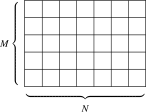
\includegraphics[width=0.3\textwidth]{imgs/matriz}
\caption{Matriz de {\it pixels} utilizada na Questão 6.}
\label{fig:matriz}
\end{figure}

\begin{itemize}
    \item [a)] Qual será o tamanho de um arquivo ({\bf em KBytes}) dessa imagem
sabendo que esta possui 60 linhas ($M = 60$) $\times$ 90 colunas ($N = 90$)?
\end{itemize}

Como a matriz tem dimensão $60 \times 90$, então, no total há 5400 {\it pixels}.
Se cada {\it pixel} é representado por 4 Bytes, então o tamanho final será
21.600 Bytes $\approx$ 21,09 KBytes.

\begin{itemize}
    \item [b)] Deseja-se comprimir esta imagem sem que haja perda da informação.
Mas, para isso a imagem deve ser antes dividida em partes menores de $6 \times
9$ {\it pixels}. Em quantas partes essa imagem será decomposta? Qual será o
tamanho ({\bf em Bytes}) de cada uma dessas partes antes de passar pelo
algoritmo de compressão?
\end{itemize}

A imagem será decomposta em 100 partes idênticas de 54 {\it pixels}. O tamanho
de cada parte será então $54 \times 4\ \text{Bytes} = 216\ \text{Bytes}$.

\begin{itemize}
    \item [c)] Se cada parte da alternativa {\it b} sofrer uma compressão de
20\%, qual será o tamanho final ({\bf em KBytes}) do arquivo comprimido?
\end{itemize}

Como as partes são idênticas, então a compressão de 20\% pode ser considerada
sobre o arquivo final. Logo, com uma compressão de 20\%, o tamanho final do
arquivo será $(1-0,2)\times 21,09 = 16,872\ \text{KBytes}$.

\pagebreak

\end{document}
